\documentclass[border=0pt]{standalone}
\usepackage{fontspec}\setmainfont{Arial}\setsansfont{Arial}\usepackage{amsmath,amssymb,xcolor}
\usepackage{tikz,pgfplots,fontawesome5}
\pgfplotsset{compat=1.18}
\usetikzlibrary{plotmarks,arrows.meta,calc,positioning,shapes.callouts,backgrounds,fit}
\pgfsetplotmarksize{1.7pt}
\tikzset{every picture/.append style={font=\sffamily\scriptsize},
  card/.style={rounded corners=2pt,draw=black!18,fill=black!2,inner sep=3pt,align=left},
  chip/.style={rounded corners=1.5pt,inner sep=1.5pt,font=\sffamily\tiny\bfseries,text=white},
  panel/.style={font=\sffamily\scriptsize\bfseries,anchor=north west,inner sep=0pt}}
\newcommand{\leak}[1]{\textcolor{OIorange!85!black}{\textbf{#1}}}
\definecolor{OIblue}{HTML}{5B7FAF}\definecolor{OIorange}{HTML}{D2876C}\definecolor{OIgreen}{HTML}{68A595}
\definecolor{OIsky}{HTML}{9CC2DD}\definecolor{OIpurple}{HTML}{B497B6}\definecolor{OIgray}{HTML}{9A9A9A}
\begin{document}
\begin{tikzpicture}[x=0.88cm,y=0.94cm]
\node[panel] at (-1.95,3.85) {(a) Net use by channel (pp)};
\node[font=\sffamily\tiny,align=center,anchor=south] at (0.30,3.02) {{\color{OIorange}\faDeaf}\\Hear};
\node[font=\sffamily\tiny,align=center,anchor=south] at (0.90,3.02) {{\color{OIorange}\faLanguage}\\Unde.};
\node[font=\sffamily\tiny,align=center,anchor=south] at (1.50,3.02) {{\color{OIorange}\faEyeSlash}\\See};
\node[font=\sffamily\tiny,align=center,anchor=south] at (2.10,3.02) {{\color{OIorange}\faEnvelope}\\Receive};
\node[anchor=east,font=\sffamily\tiny] at (-0.05,2.878) {Nemotron-3-Nano};
\fill[OIorange!84!white] (0.010,2.766) rectangle (0.590,2.990);\node[text=black!80,font=\sffamily\tiny] at (0.300,2.878) {99};
\fill[OIorange!56!white] (0.610,2.766) rectangle (1.190,2.990);\node[text=black!80,font=\sffamily\tiny] at (0.900,2.878) {66};
\fill[OIorange!83!white] (1.210,2.766) rectangle (1.790,2.990);\node[text=black!80,font=\sffamily\tiny] at (1.500,2.878) {98};
\fill[OIorange!84!white] (1.810,2.766) rectangle (2.390,2.990);\node[text=black!80,font=\sffamily\tiny] at (2.100,2.878) {99};
\node[anchor=east,font=\sffamily\tiny] at (-0.05,2.634) {Qwen3.5-9B};
\fill[OIorange!83!white] (0.010,2.522) rectangle (0.590,2.746);\node[text=black!80,font=\sffamily\tiny] at (0.300,2.634) {97};
\fill[OIorange!44!white] (0.610,2.522) rectangle (1.190,2.746);\node[text=black!80,font=\sffamily\tiny] at (0.900,2.634) {51};
\fill[OIorange!82!white] (1.210,2.522) rectangle (1.790,2.746);\node[text=black!80,font=\sffamily\tiny] at (1.500,2.634) {97};
\fill[OIorange!82!white] (1.810,2.522) rectangle (2.390,2.746);\node[text=black!80,font=\sffamily\tiny] at (2.100,2.634) {96};
\node[anchor=east,font=\sffamily\tiny] at (-0.05,2.390) {gpt-oss-20b};
\fill[OIorange!81!white] (0.010,2.278) rectangle (0.590,2.502);\node[text=black!80,font=\sffamily\tiny] at (0.300,2.390) {95};
\fill[OIorange!32!white] (0.610,2.278) rectangle (1.190,2.502);\node[text=black!80,font=\sffamily\tiny] at (0.900,2.390) {37};
\fill[OIorange!78!white] (1.210,2.278) rectangle (1.790,2.502);\node[text=black!80,font=\sffamily\tiny] at (1.500,2.390) {91};
\fill[OIorange!75!white] (1.810,2.278) rectangle (2.390,2.502);\node[text=black!80,font=\sffamily\tiny] at (2.100,2.390) {89};
\node[anchor=east,font=\sffamily\tiny] at (-0.05,2.146) {Phi-4};
\fill[OIorange!83!white] (0.010,2.034) rectangle (0.590,2.258);\node[text=black!80,font=\sffamily\tiny] at (0.300,2.146) {97};
\fill[OIorange!12!white] (0.610,2.034) rectangle (1.190,2.258);\node[text=black!80,font=\sffamily\tiny] at (0.900,2.146) {14};
\fill[OIorange!79!white] (1.210,2.034) rectangle (1.790,2.258);\node[text=black!80,font=\sffamily\tiny] at (1.500,2.146) {93};
\fill[OIorange!83!white] (1.810,2.034) rectangle (2.390,2.258);\node[text=black!80,font=\sffamily\tiny] at (2.100,2.146) {98};
\node[anchor=east,font=\sffamily\tiny] at (-0.05,1.902) {Falcon-H1-34B};
\fill[OIorange!54!white] (0.010,1.790) rectangle (0.590,2.014);\node[text=black!80,font=\sffamily\tiny] at (0.300,1.902) {64};
\fill[OIorange!64!white] (0.610,1.790) rectangle (1.190,2.014);\node[text=black!80,font=\sffamily\tiny] at (0.900,1.902) {75};
\fill[OIorange!47!white] (1.210,1.790) rectangle (1.790,2.014);\node[text=black!80,font=\sffamily\tiny] at (1.500,1.902) {55};
\fill[OIorange!83!white] (1.810,1.790) rectangle (2.390,2.014);\node[text=black!80,font=\sffamily\tiny] at (2.100,1.902) {98};
\node[anchor=east,font=\sffamily\tiny] at (-0.05,1.659) {GLM-4.7-Flash};
\fill[OIorange!74!white] (0.010,1.547) rectangle (0.590,1.770);\node[text=black!80,font=\sffamily\tiny] at (0.300,1.659) {87};
\fill[OIorange!60!white] (0.610,1.547) rectangle (1.190,1.770);\node[text=black!80,font=\sffamily\tiny] at (0.900,1.659) {71};
\fill[OIorange!56!white] (1.210,1.547) rectangle (1.790,1.770);\node[text=black!80,font=\sffamily\tiny] at (1.500,1.659) {66};
\fill[OIorange!45!white] (1.810,1.547) rectangle (2.390,1.770);\node[text=black!80,font=\sffamily\tiny] at (2.100,1.659) {53};
\node[anchor=east,font=\sffamily\tiny] at (-0.05,1.415) {Seed-OSS-36B};
\fill[OIorange!51!white] (0.010,1.303) rectangle (0.590,1.527);\node[text=black!80,font=\sffamily\tiny] at (0.300,1.415) {60};
\fill[OIorange!50!white] (0.610,1.303) rectangle (1.190,1.527);\node[text=black!80,font=\sffamily\tiny] at (0.900,1.415) {59};
\fill[OIorange!45!white] (1.210,1.303) rectangle (1.790,1.527);\node[text=black!80,font=\sffamily\tiny] at (1.500,1.415) {53};
\fill[OIorange!51!white] (1.810,1.303) rectangle (2.390,1.527);\node[text=black!80,font=\sffamily\tiny] at (2.100,1.415) {60};
\node[anchor=east,font=\sffamily\tiny] at (-0.05,1.171) {Gemma-4-12B};
\fill[OIorange!85!white] (0.010,1.059) rectangle (0.590,1.283);\node[text=black!80,font=\sffamily\tiny] at (0.300,1.171) {99};
\fill[OIorange!12!white] (0.610,1.059) rectangle (1.190,1.283);\node[text=black!80,font=\sffamily\tiny] at (0.900,1.171) {14};
\fill[OIorange!20!white] (1.210,1.059) rectangle (1.790,1.283);\node[text=black!80,font=\sffamily\tiny] at (1.500,1.171) {24};
\fill[OIorange!67!white] (1.810,1.059) rectangle (2.390,1.283);\node[text=black!80,font=\sffamily\tiny] at (2.100,1.171) {79};
\node[anchor=east,font=\sffamily\tiny] at (-0.05,0.927) {Mistral-Small-24B};
\fill[OIorange!81!white] (0.010,0.815) rectangle (0.590,1.039);\node[text=black!80,font=\sffamily\tiny] at (0.300,0.927) {96};
\fill[OIorange!1!white] (0.610,0.815) rectangle (1.190,1.039);\node[text=black!80,font=\sffamily\tiny] at (0.900,0.927) {2};
\fill[OIorange!26!white] (1.210,0.815) rectangle (1.790,1.039);\node[text=black!80,font=\sffamily\tiny] at (1.500,0.927) {31};
\fill[OIorange!71!white] (1.810,0.815) rectangle (2.390,1.039);\node[text=black!80,font=\sffamily\tiny] at (2.100,0.927) {83};
\node[anchor=east,font=\sffamily\tiny] at (-0.05,0.683) {Qwen3.8-27B};
\fill[OIorange!19!white] (0.010,0.571) rectangle (0.590,0.795);\node[text=black!80,font=\sffamily\tiny] at (0.300,0.683) {22};
\fill[OIorange!2!white] (0.610,0.571) rectangle (1.190,0.795);\node[text=black!80,font=\sffamily\tiny] at (0.900,0.683) {3};
\fill[OIorange!35!white] (1.210,0.571) rectangle (1.790,0.795);\node[text=black!80,font=\sffamily\tiny] at (1.500,0.683) {41};
\fill[OIorange!13!white] (1.810,0.571) rectangle (2.390,0.795);\node[text=black!80,font=\sffamily\tiny] at (2.100,0.683) {15};
\node[anchor=east,font=\sffamily\tiny] at (-0.05,0.439) {Gemma-4-31B};
\fill[OIorange!5!white] (0.010,0.327) rectangle (0.590,0.551);\node[text=black!80,font=\sffamily\tiny] at (0.300,0.439) {5};
\fill[OIorange!0!white] (0.610,0.327) rectangle (1.190,0.551);\node[text=black!80,font=\sffamily\tiny] at (0.900,0.439) {0};
\fill[OIorange!14!white] (1.210,0.327) rectangle (1.790,0.551);\node[text=black!80,font=\sffamily\tiny] at (1.500,0.439) {16};
\fill[OIorange!19!white] (1.810,0.327) rectangle (2.390,0.551);\node[text=black!80,font=\sffamily\tiny] at (2.100,0.439) {22};
\node[anchor=east,font=\sffamily\tiny\bfseries] at (-0.05,0.135) {Mean};
\fill[OIorange!64!white] (0.010,0.023) rectangle (0.590,0.247);\node[text=black!80,font=\sffamily\tiny\bfseries] at (0.300,0.135) {75};
\fill[OIorange!30!white] (0.610,0.023) rectangle (1.190,0.247);\node[text=black!80,font=\sffamily\tiny\bfseries] at (0.900,0.135) {36};
\fill[OIorange!51!white] (1.210,0.023) rectangle (1.790,0.247);\node[text=black!80,font=\sffamily\tiny\bfseries] at (1.500,0.135) {61};
\fill[OIorange!61!white] (1.810,0.023) rectangle (2.390,0.247);\node[text=black!80,font=\sffamily\tiny\bfseries] at (2.100,0.135) {72};
\begin{scope}[xshift=2.772cm]
\node[panel] at (0,3.85) {(b) Access format};
\draw[black!9] (0.156,0)--(0.156,3.0);
\draw[black!9] (0.778,0)--(0.778,3.0);
\draw[black!9] (1.400,0)--(1.400,3.0);
\draw[black!9] (2.022,0)--(2.022,3.0);
\draw[black!9] (2.644,0)--(2.644,3.0);
\draw[black!45,line width=.4pt] (0,3.0)--(0,0)--(2.8,0);
\node[anchor=north,font=\sffamily\tiny,text=black!70,inner sep=1.5pt] at (0.156,0) {-40};
\node[anchor=north,font=\sffamily\tiny,text=black!70,inner sep=1.5pt] at (0.778,0) {-20};
\node[anchor=north,font=\sffamily\tiny,text=black!70,inner sep=1.5pt] at (1.400,0) {0};
\node[anchor=north,font=\sffamily\tiny,text=black!70,inner sep=1.5pt] at (2.022,0) {20};
\node[anchor=north,font=\sffamily\tiny,text=black!70,inner sep=1.5pt] at (2.644,0) {40};
\node[anchor=north,font=\sffamily\scriptsize] at (1.4,-0.3) {change in net use (pp)};
\draw[black!55] (1.400,0)--(1.400,3.0);
\node[anchor=east,font=\footnotesize,text=OIorange] at (-0.02,2.625) {\faDeaf};
\fill[OIblue] (1.400,2.650) rectangle (1.945,2.820);\draw[black!60,line width=.35pt] (1.865,2.735)--(2.025,2.735);
\fill[OIgreen] (1.400,2.430) rectangle (0.230,2.600);\draw[black!60,line width=.35pt] (0.115,2.515)--(0.345,2.515);
\node[anchor=east,font=\footnotesize,text=OIorange] at (-0.02,1.875) {\faLanguage};
\fill[OIblue] (1.400,1.900) rectangle (2.290,2.070);\draw[black!60,line width=.35pt] (2.193,1.985)--(2.390,1.985);
\fill[OIgreen] (1.400,1.680) rectangle (1.276,1.850);\draw[black!60,line width=.35pt] (1.150,1.765)--(1.397,1.765);
\node[anchor=east,font=\footnotesize,text=OIorange] at (-0.02,1.125) {\faEyeSlash};
\fill[OIblue] (1.400,1.150) rectangle (2.422,1.320);\draw[black!60,line width=.35pt] (2.302,1.235)--(2.546,1.235);
\fill[OIgreen] (1.400,0.930) rectangle (0.855,1.100);\draw[black!60,line width=.35pt] (0.699,1.015)--(0.985,1.015);
\node[anchor=east,font=\footnotesize,text=OIorange] at (-0.02,0.375) {\faEnvelope};
\fill[OIblue] (1.400,0.400) rectangle (1.506,0.570);\draw[black!60,line width=.35pt] (1.418,0.485)--(1.597,0.485);
\fill[OIgreen] (1.400,0.180) rectangle (0.222,0.350);\draw[black!60,line width=.35pt] (0.113,0.265)--(0.339,0.265);
\fill[OIblue] (0.05,-0.92) rectangle (0.2,-0.8);\node[anchor=west,font=\sffamily\tiny] at (0.22,-0.86) {membership list};
\fill[OIgreen] (0.05,-1.17) rectangle (0.2,-1.05);\node[anchor=west,font=\sffamily\tiny] at (0.22,-1.11) {flag + prose rule};
\end{scope}
\begin{scope}[xshift=5.940cm]
\node[panel] at (-0.4,3.85) {(c) Persistence};
\draw[black!9] (0,0.000)--(2.2,0.000);
\draw[black!9] (0,0.750)--(2.2,0.750);
\draw[black!9] (0,1.500)--(2.2,1.500);
\draw[black!9] (0,2.250)--(2.2,2.250);
\draw[black!9] (0,3.000)--(2.2,3.000);
\draw[black!45,line width=.4pt] (0,3.0)--(0,0)--(2.2,0);
\node[anchor=north,font=\sffamily\tiny,text=black!70,inner sep=1.5pt] at (0.000,0) {0};
\node[anchor=north,font=\sffamily\tiny,text=black!70,inner sep=1.5pt] at (1.100,0) {2};
\node[anchor=north,font=\sffamily\tiny,text=black!70,inner sep=1.5pt] at (2.200,0) {4};
\node[anchor=east,font=\sffamily\tiny,text=black!70,inner sep=1.5pt] at (0,0.000) {0};
\node[anchor=east,font=\sffamily\tiny,text=black!70,inner sep=1.5pt] at (0,0.750) {25};
\node[anchor=east,font=\sffamily\tiny,text=black!70,inner sep=1.5pt] at (0,1.500) {50};
\node[anchor=east,font=\sffamily\tiny,text=black!70,inner sep=1.5pt] at (0,2.250) {75};
\node[anchor=east,font=\sffamily\tiny,text=black!70,inner sep=1.5pt] at (0,3.000) {100};
\node[anchor=north,font=\sffamily\scriptsize] at (1.1,-0.3) {neutral exchanges};
\node[anchor=south,rotate=90,font=\sffamily\scriptsize] at (-0.55,1.5) {net use (pp)};
\draw[OIorange,line width=.9pt] (0.000,2.074)--(1.100,2.062)--(2.200,2.133);
\path[OIorange] plot[mark=triangle*] coordinates {(0.000,2.074)};
\path[OIorange] plot[mark=triangle*] coordinates {(1.100,2.062)};
\path[OIorange] plot[mark=triangle*] coordinates {(2.200,2.133)};
\draw[OIblue,line width=.9pt] (0.000,1.277)--(1.100,1.582)--(2.200,1.746);
\path[OIblue] plot[mark=*] coordinates {(0.000,1.277)};
\path[OIblue] plot[mark=*] coordinates {(1.100,1.582)};
\path[OIblue] plot[mark=*] coordinates {(2.200,1.746)};
\draw[OIpurple,line width=.9pt] (0.000,1.664)--(1.100,1.500)--(2.200,1.523);
\path[OIpurple] plot[mark=square*] coordinates {(0.000,1.664)};
\path[OIpurple] plot[mark=square*] coordinates {(1.100,1.500)};
\path[OIpurple] plot[mark=square*] coordinates {(2.200,1.523)};
\draw[OIsky,line width=.9pt] (0.000,2.039)--(1.100,2.051)--(2.200,2.086);
\path[OIsky] plot[mark=diamond*] coordinates {(0.000,2.039)};
\path[OIsky] plot[mark=diamond*] coordinates {(1.100,2.051)};
\path[OIsky] plot[mark=diamond*] coordinates {(2.200,2.086)};
\node[anchor=west,font=\sffamily\tiny,text=OIpurple] at (2.320,1.523) {See};
\node[anchor=west,font=\sffamily\tiny,text=OIblue] at (2.320,1.746) {Understand};
\node[anchor=west,font=\sffamily\tiny,text=OIsky] at (2.320,2.086) {Receive};
\node[anchor=west,font=\sffamily\tiny,text=OIorange] at (2.320,2.286) {Hear};
\draw[OIgreen,line width=.9pt,densely dashed] (0,0.000)--(2.2,0.000);\node[anchor=south west,font=\sffamily\tiny,text=OIgreen] at (0.05,0.000) {character view, all channels};
\end{scope}
\begin{scope}[xshift=9.636cm]
\node[panel] at (-0.35,3.85) {(d) Choosing where to search};
\draw[black!9] (0.000,0)--(0.000,3.0);
\draw[black!9] (0.688,0)--(0.688,3.0);
\draw[black!9] (1.375,0)--(1.375,3.0);
\draw[black!9] (2.062,0)--(2.062,3.0);
\draw[black!9] (2.750,0)--(2.750,3.0);
\draw[black!45,line width=.4pt] (0,3.0)--(0,0)--(2.75,0);
\node[anchor=north,font=\sffamily\tiny,text=black!70,inner sep=1.5pt] at (0.000,0) {0};
\node[anchor=north,font=\sffamily\tiny,text=black!70,inner sep=1.5pt] at (0.688,0) {20};
\node[anchor=north,font=\sffamily\tiny,text=black!70,inner sep=1.5pt] at (1.375,0) {40};
\node[anchor=north,font=\sffamily\tiny,text=black!70,inner sep=1.5pt] at (2.062,0) {60};
\node[anchor=north,font=\sffamily\tiny,text=black!70,inner sep=1.5pt] at (2.750,0) {80};
\node[anchor=north,font=\sffamily\scriptsize] at (1.375,-0.3) {change in choosing A (pp)};
\node[anchor=east,font=\footnotesize,text=OIorange] at (-0.02,2.625) {\faDeaf};
\fill[OIorange] (0,2.650) rectangle (2.175,2.820);\draw[black!60,line width=.35pt] (1.853,2.735)--(2.444,2.735);
\fill[OIgreen] (0,2.430) rectangle (0.027,2.600);\draw[black!60,line width=.35pt] (0.000,2.515)--(0.081,2.515);
\node[anchor=east,font=\footnotesize,text=OIorange] at (-0.02,1.875) {\faLanguage};
\fill[OIorange] (0,1.900) rectangle (1.880,2.070);\draw[black!60,line width=.35pt] (1.638,1.985)--(2.095,1.985);
\fill[OIgreen] (0,1.680) rectangle (0.000,1.850);\draw[black!60,line width=.35pt] (0.000,1.765)--(0.000,1.765);
\node[anchor=east,font=\footnotesize,text=OIorange] at (-0.02,1.125) {\faEyeSlash};
\fill[OIorange] (0,1.150) rectangle (1.692,1.320);\draw[black!60,line width=.35pt] (1.477,1.235)--(1.880,1.235);
\fill[OIgreen] (0,0.930) rectangle (0.000,1.100);\draw[black!60,line width=.35pt] (0.000,1.015)--(0.000,1.015);
\node[anchor=east,font=\footnotesize,text=OIorange] at (-0.02,0.375) {\faEnvelope};
\fill[OIorange] (0,0.400) rectangle (1.907,0.570);\draw[black!60,line width=.35pt] (1.611,0.485)--(2.202,0.485);
\fill[OIgreen] (0,0.180) rectangle (0.000,0.350);\draw[black!60,line width=.35pt] (0.000,0.265)--(0.000,0.265);
\fill[OIorange] (0.05,-0.92) rectangle (0.2,-0.8);\node[anchor=west,font=\sffamily\tiny] at (0.22,-0.86) {full context};
\fill[OIgreen] (0.05,-1.17) rectangle (0.2,-1.05);\node[anchor=west,font=\sffamily\tiny] at (0.22,-1.11) {character view};
\end{scope}
\end{tikzpicture}
\end{document}
